\documentclass[journal]{vgtc}                % final (journal style)
%\documentclass[review,journal]{vgtc}         % review (journal style)
%\documentclass[widereview]{vgtc}             % wide-spaced review
%\documentclass[preprint,journal]{vgtc}       % preprint (journal style)
%\documentclass[electronic,journal]{vgtc}     % electronic version, journal

%% Uncomment one of the lines above depending on where your paper is
%% in the conference process. ``review'' and ``widereview'' are for review
%% submission, ``preprint'' is for pre-publication, and the final version
%% doesn't use a specific qualifier. Further, ``electronic'' includes
%% hyperreferences for more convenient online viewing.

%% Please use one of the ``review'' options in combination with the
%% assigned online id (see below) ONLY if your paper uses a double blind
%% review process. Some conferences, like IEEE Vis and InfoVis, have NOT
%% in the past.

%% Please note that the use of figures other than the optional teaser is not permitted on the first page
%% of the journal version.  Figures should begin on the second page and be
%% in CMYK or Grey scale format, otherwise, colour shifting may occur
%% during the printing process.  Papers submitted with figures other than the optional teaser on the
%% first page will be refused.

%% These three lines bring in essential packages: ``mathptmx'' for Type 1
%% typefaces, ``graphicx'' for inclusion of EPS figures. and ``times''
%% for proper handling of the times font family.
%\usepackage{natbib}
\usepackage{mathptmx}
\usepackage{graphicx}
\usepackage{times}
\usepackage{amsmath}
\usepackage{multirow}
\usepackage{url}
\usepackage[table]{xcolor}

\renewcommand\floatpagefraction{1}

%% We encourage the use of mathptmx for consistent usage of times font
%% throughout the proceedings. However, if you encounter conflicts
%% with other math-related packages, you may want to disable it.

%% If you are submitting a paper to a conference for review with a double
%% blind reviewing process, please replace the value ``0'' below with your
%% OnlineID. Otherwise, you may safely leave it at ``0''.
\onlineid{0}

%% declare the category of your paper, only shown in review mode
\vgtccategory{Research}

%% allow for this line if you want the electronic option to work properly
\vgtcinsertpkg

%% In preprint mode you may define your own headline.
%\preprinttext{To appear in an IEEE VGTC sponsored conference.}

%% Paper title.

\title{Common Angle Plots as perception-true visualizations of categorical associations}

%% This is how authors are specified in the journal style

%% indicate IEEE Member or Student Member in form indicated below
\author{Heike Hofmann, Marie Vendettuoli}
\authorfooter{
%% insert punctuation at end of each item
\item
 Heike Hofmann is an associate professor in Statistics and faculty member in the Human Computer Interaction program at Iowa State University, E-mail: hofmann@iastate.edu.
\item
Marie Vendettuoli is a graduate student at Iowa State University, with majors in Human Computer Interaction and Bioinfomatics \& Computational Biology. She is a past IGERT Fellow and currently interns with the Statistics section at USDA.  E-mail: mariev@iastate.edu.
}

%other entries to be set up for journal
\shortauthortitle{Hofmann \MakeLowercase{\textit{et al.}}: Common Angle Plots}
%\shortauthortitle{Firstauthor \MakeLowercase{\textit{et al.}}: Paper Title}

%% Abstract section.
\abstract{
Visualizations are great tools of communications - they summarize findings and quickly convey main messages to our audience. As designers of charts we have to make sure that information is shown with a minimum of distortion. We have to also consider illusions and other perceptual  limitations of our audience. In this paper we discuss  the effect and strength of the  line width illusion,  a M\"uller-Lyer type illusion, on designs related to displaying associations between categorical variables. Parallel sets and hammock plots are both affected by line width illusions. We  introduce the common-angle plot as an alternative method for displaying categorical data in a manner that minimizes the effect from perceptual illusions.
Finally, we present results from user studies as evidence that common angle charts resolve  problems with the line width illusion.
} % end of abstract

%% Keywords that describe your work. Will show as 'Index Terms' in journal
%% please capitalize first letter and insert punctuation after last keyword
\keywords{Linewidth illusion, Data Visualization, High-dimensional Displays, Parallel Sets, Hammock Plots, M\"uller-Lyer Illusion.}

%% ACM Computing Classification System (CCS). 
%% See <http://www.acm.org/class/1998/> for details.
%% The ``\CCScat'' command takes four arguments.

\CCScatlist{ % not used in journal version
  \category{H.5.2}{Information Interfaces and Presentation}{ User Interfaces --- Graphical user interfaces (GUI), Interaction styles, Screen design, Evaluation/methodology}
  \CCScat{I.6.8}{Computing Methodologies}%
  {Simulation and Modeling}{Visual Simulation};
}

\graphicspath{{images/}}
\definecolor{LightGrey}{gray}{0.9}

%% Uncomment below to include a teaser figure.
\teaser{
\centering
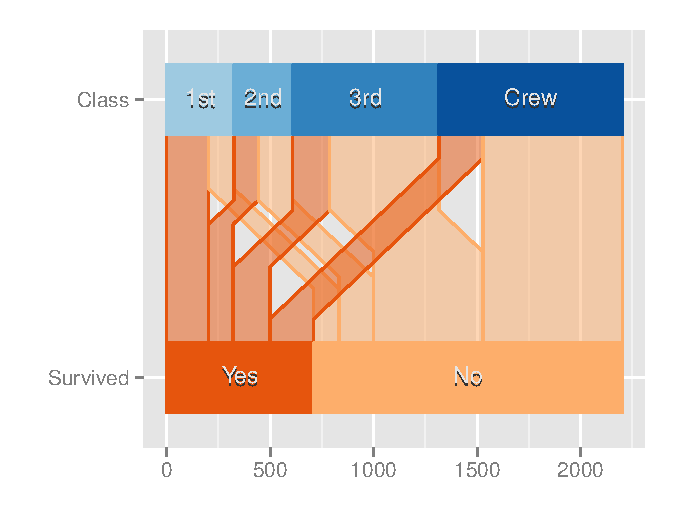
\includegraphics[height=1.5in]{ca-titanic-teaser.pdf}\hspace{0.01\linewidth}
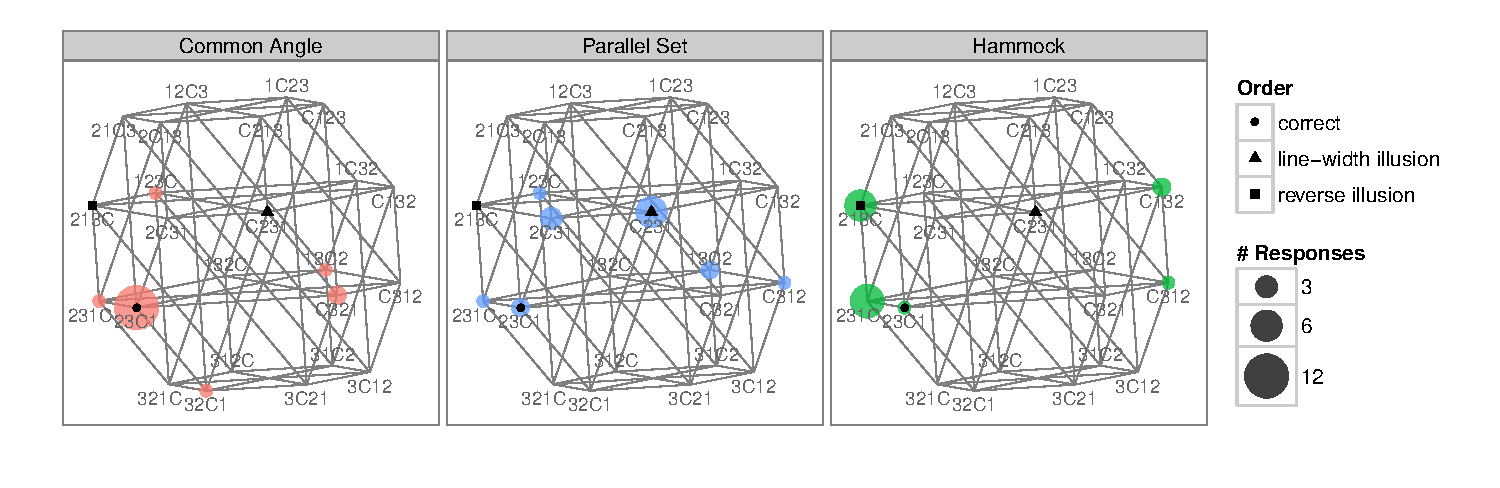
\includegraphics[height=1.5in]{cubes.pdf}
%\includegraphics[width=16cm]{CypressView.eps}
\caption{Who survived on the Titanic? Common Angle plot of survival by class (left). On the right, graphs showing survey results with answers.}
}

%% Uncomment below to disable the manuscript note
%\renewcommand{\manuscriptnotetxt}{}

%% Copyright space is enabled by default as required by guidelines.
%% It is disabled by the 'review' option or via the following command:
% \nocopyrightspace

%%%%%%%%%%%%%%%%%%%%%%%%%%%%%%%%%%%%%%%%%%%%%%%%%%%%%%%%%%%%%%%%
%%%%%%%%%%%%%%%%%%%%%% START OF THE PAPER %%%%%%%%%%%%%%%%%%%%%%
%%%%%%%%%%%%%%%%%%%%%%%%%%%%%%%%%%%%%%%%%%%%%%%%%%%%%%%%%%%%%%%%%

\begin{document}

%% The ``\maketitle'' command must be the first command after the
%% ``\begin{document}'' command. It prepares and prints the title block.

%% the only exception to this rule is the \firstsection command
\firstsection{Introduction}

\maketitle

% !TEX root = bare_jrnl_compsoc.tex


\section{Introduction}
% The very first letter is a 2 line initial drop letter followed
% by the rest of the first word in caps.
% 
% form to use if the first word consists of a single letter:
% \IEEEPARstart{A}{demo} file is ....
% 
% form to use if you need the single drop letter followed by
% normal text (unknown if ever used by IEEE):
% \IEEEPARstart{A}{}demo file is ....
% 
% Some journals put the first two words in caps:
% \IEEEPARstart{T}{his demo} file is ....
% 
% Here we have the typical use of a "T" for an initial drop letter
% and "HIS" in caps to complete the first word.
\IEEEPARstart{A}{ well-designed} graph is a powerful tool 
that transends barriers of language to
communicate complex concepts from author to audience. It becomes a 
problem if readers are unable to easily extract the main message, especially
when distortion is encoded. The source of a distortion may be due to 
intrinsic deformities in the graph or simply the perceptual limitations of
the audience. Examples include Tufte's \emph{Lie-Factor} \cite[p. 57--69]{tufte} in which the proportion of the physical space occupied by the graphic is 
inconsistent with underlying data; calculated ratio (of proportions) less than one indicate 
underrepresentation. Another example is the M\"{u}ller-Lyer family of illusions such as the sine wave, where viewers perceive extents at the curves to be of different height than in the straight regions even though all regions were of the same height \cite{day:1991}.

Regardless of the cause of distortion, the graph author has a duty to create visualizations that
 allows readers to extract an accurate interpretation of the underlying data. The \emph{Lie-Factor}
provides a quantitative method to evaluate distortion due to graph deformities. In order to ascertain the
impact of distortion due to perceptual limits, usability studies provide empirical evidence supporting 
underlying metaphorical models, both known and unpredicted.  




Parallel sets (parsets)  \cite{kosara:2006}, a graphical method  for visualizing multivariate categorical data, presents a case of unspecified distortion due to perceptual limits . Since initial publication, parsets have spread to mass media outlets  \cite{eagereyes, bostock:2012, bbc:2009}, multiple technical implementations \cite{eagereyes, d3, davies} and is a reputable resource for further academic work (\cite{kosara:2006} has 70 citations per Google scholar). While retaining the %independent 
ability to visualize a large number of dimensions simultaneously that is the parallel coordinates' hallmark trade, parsets introduce the frequency scale that is a well-known feature of other categorical displays such as barcharts or mosaic plots \cite{hartigan:1981, friendly:1992, hofmann:2000, theus:1997}.
% Initially, frequencies of categories  were displayed as stacked boxes; in  later versions of parallel sets the boxes are reduced to simple lines \cite{parsetredesign}. Various implementations of parallel sets exist besides the original Java version of Eagereyes \cite{eagereyes}, e.g.  J Davies introduced a d3 \cite{d3} version in  \cite{davies}.  


\begin{figure}[hbtp]
\centering
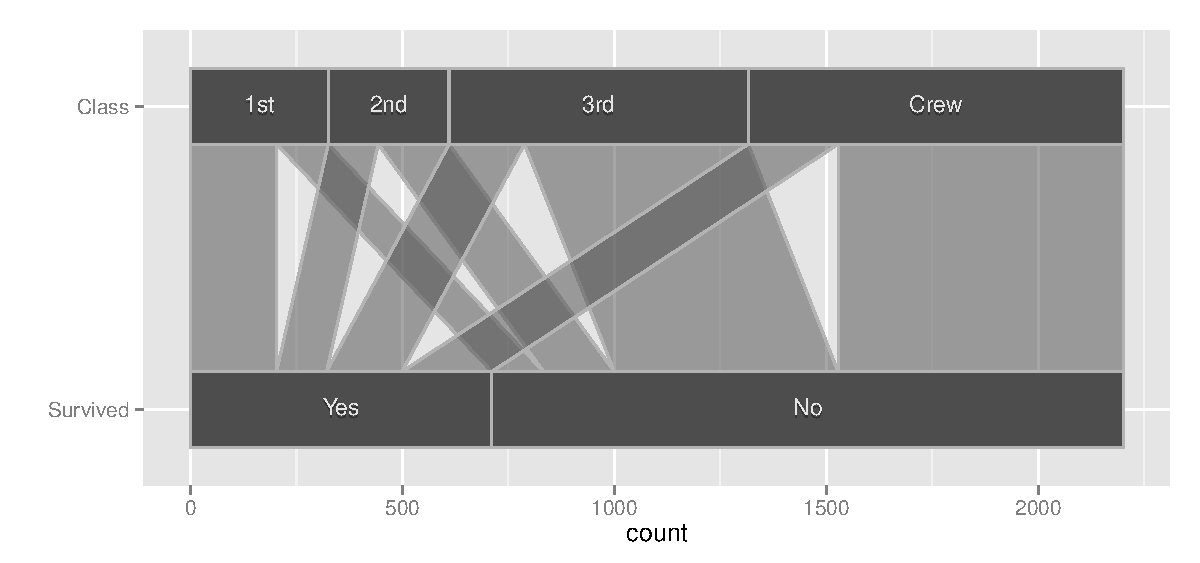
\includegraphics[width=.9\linewidth]{images/parset-titanic}
\caption{\label{question1a} Parallel sets plot showing the relationship between survival of the sinking of the HMS Titanic and class membership. }
\end{figure}
%XXX Description of parallel sets - and example


%%XXX PS and line-width illusion
Figure \ref{question1a} gives an example for a two dimensional parallel sets plot investigating the relationship between class status and survival on board the HMS Titanic  \cite{dawson:1995}. Class status is recorded as either crew member or passengers in  first, second, or third class.  The top bar in figure \ref{question1a} shows the  variable Class. The bottom bar shows survival  as yes and no. Between the bars lines are drawn to visualize the relationship between class membership and  survival. 
  Based on the number of survivor and non survivors
  these bands are drawn from each class, and their (horizontal) width is proportional to the number of people they represent. A reasonable task would be to order levels of the variable `class' by number of survivors. However, when study participants were asked to perform this task, only $12.5\%$ respondants 
selected the correct order \ref{raw}.

\begin{table}
\begin{center}
\begin{tabular}{rrrrr}
& Crew & 1st & 2nd & 3rd \\ \hline
Survivors & 212 & 203 & 118 & 178\\
Non-Survivors & 673 & 122 & 167 &  528  
\end{tabular}
\caption{Correct ordering of variable Class is: crew, first class, third class, followed by second class. }
\end{center}
\end{table}
We believe that readers view parsets they are subject to the \emph{line width illusion}, a perceptual distortion that we describe and quantify in this paper. We also propose and test \emph{common angle plots}, an alternative graphing method for visualizing multivariate categorical is not subject to the \emph{line width illusion}.
%XXX PS and line-width illusion


%
% You must have at least 2 lines in the paragraph with the drop letter
% (should never be an issue)

\section{Line width illusion}




\begin{figure}
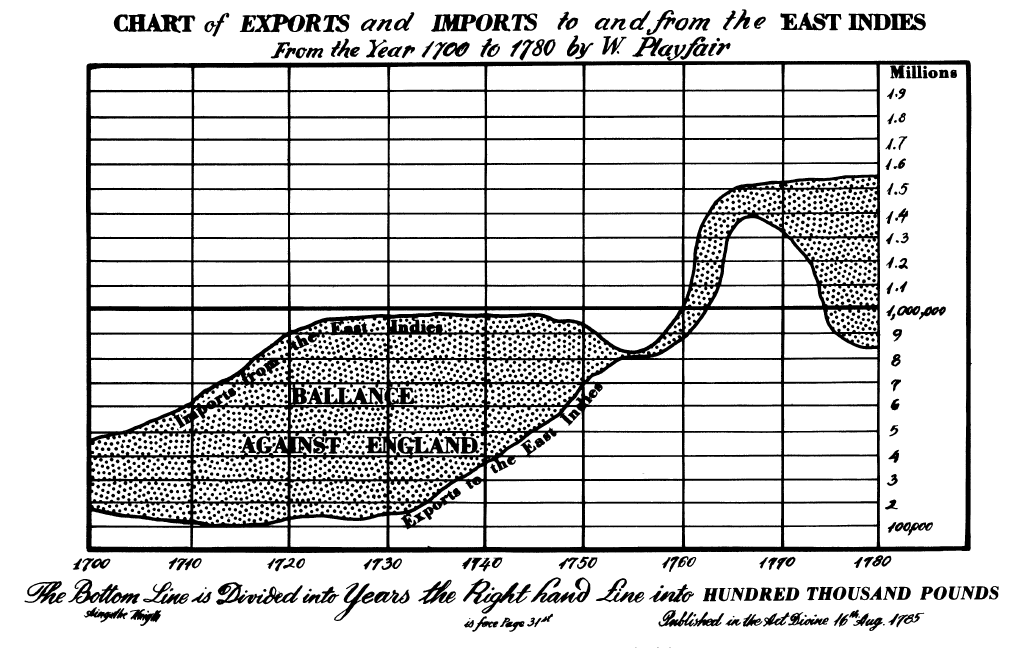
\includegraphics[width=.9\linewidth]{images/playfair_east_indies_gross}
\caption{\label{playfair}
Playfair's chart from the Commercial and Political Atlas (1786) showing the balance of trade between England and the East Indies.  In which years was the difference between imports and exports the highest? }
\end{figure}
An example of the  {\it line width illusion} is displayed in  figure  \ref{playfair}. This chart displays the balance of trade between England and the East Indies as shown by William Playfair in his Commercial and Political Atlas, 1786 \cite{playfair, playfair2}.  One purpose of this chart is to demonstrate the difference between imports and exports in a particular year and its pattern over that time frame. The difference in exports and imports is encoded as the vertical difference between the lines. When observers are asked to sketch out the difference between exports and imports  \cite{cleveland:1984}, they very often  miss the steep rise in the difference between the lines in the years between about 1755 and 1765. Figure \ref{playfair2} shows the  actual difference between imports and exports. 



\begin{figure}
\centering
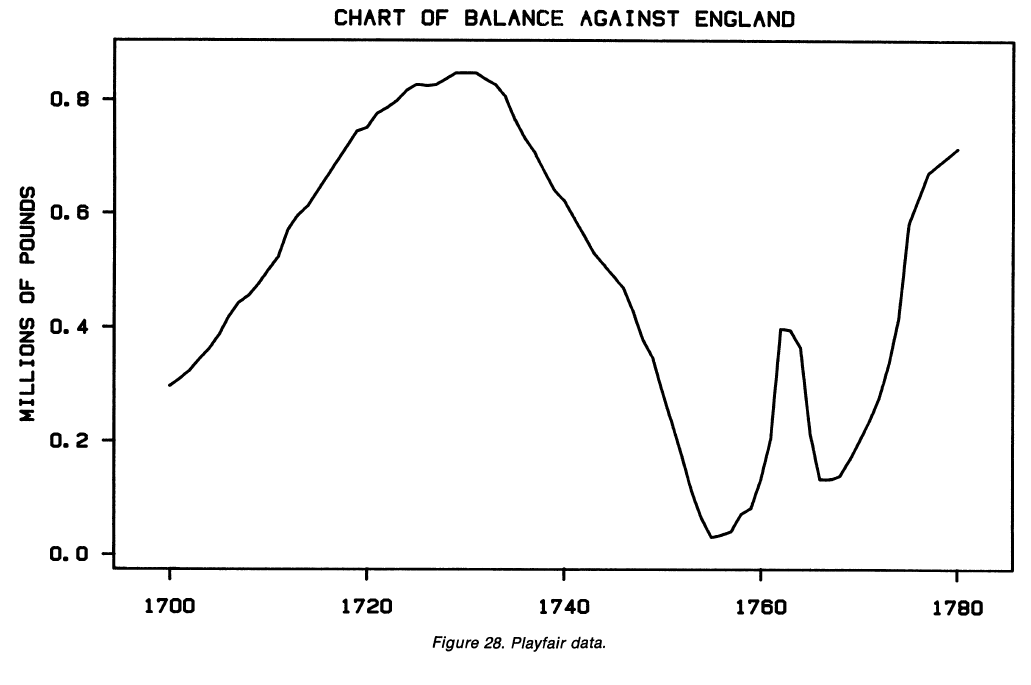
\includegraphics[width=.8\linewidth, height=.4\linewidth]{images/playfair_differenz_cleveland}
\caption{\label{playfair2}
Difference between exports and imports from England to and from the East Indies in the 18th century -- the steep rise in the difference around 1760  comes as a surprise to many viewers of the raw data in figure \ref{playfair}.  }
\end{figure}


This phenomenon  is known and widely discussed in statistical graphics literature \cite{cleveland:1984, tufte, wainer:2000, robbins:2005}. It  is due to our  tendency to assess distance between curves as the minimal (orthogonal) distance rather than the  vertical distance -- see sketch \ref{fig:linewidth} for a visual representation of both.


In the perception literature, this phenomenon is known as part of a group of geometrical optical misperceptions of a context-sensitive nature classified as M\"uller-Lyer illusions \cite{day:1991}. Interestingly, there seems to be a general agreement that this illusion exists, but a quantification of it is curiously absent from literature. 

The type of chart as shown in figure~\ref{playfair} proposed by Playfair is shown quite commonly, particular in election years -- where these kind of charts are used to enable comparisons of support for several candidates, the recommendation from literature is to avoid charts in which the audience is asked to do visual subtractions, and show these differences directly.

\subsection{Strength of  line width illusion}\label{distortion}

%The difference between perceived and actual line width 
When visually evaluating lines of thickness greater than one, the line width illusion applies, only now the {\it edges} of a single line  take on the role of the separate curves. %in the parallel sets 
As above, there is a strong preference of evaluating the width of lines orthogonal to their slopes as opposed to horizontally (see figure \ref{fig:linewidth})  needed for a correct  evaluation of parsets-style displays.

Orthogonal $w_o$ and horizontal $w_h$ line widths are related -- the orthogonal line width depends on the angle (or, equivalently, the slope) of the line:
\begin{equation}\label{adjust}
w_o = w_h \sin \theta,
\end{equation}
where $\theta$ is the angle of the line with respect to the horizontal line.

\begin{figure}[htbp]
\begin{center}
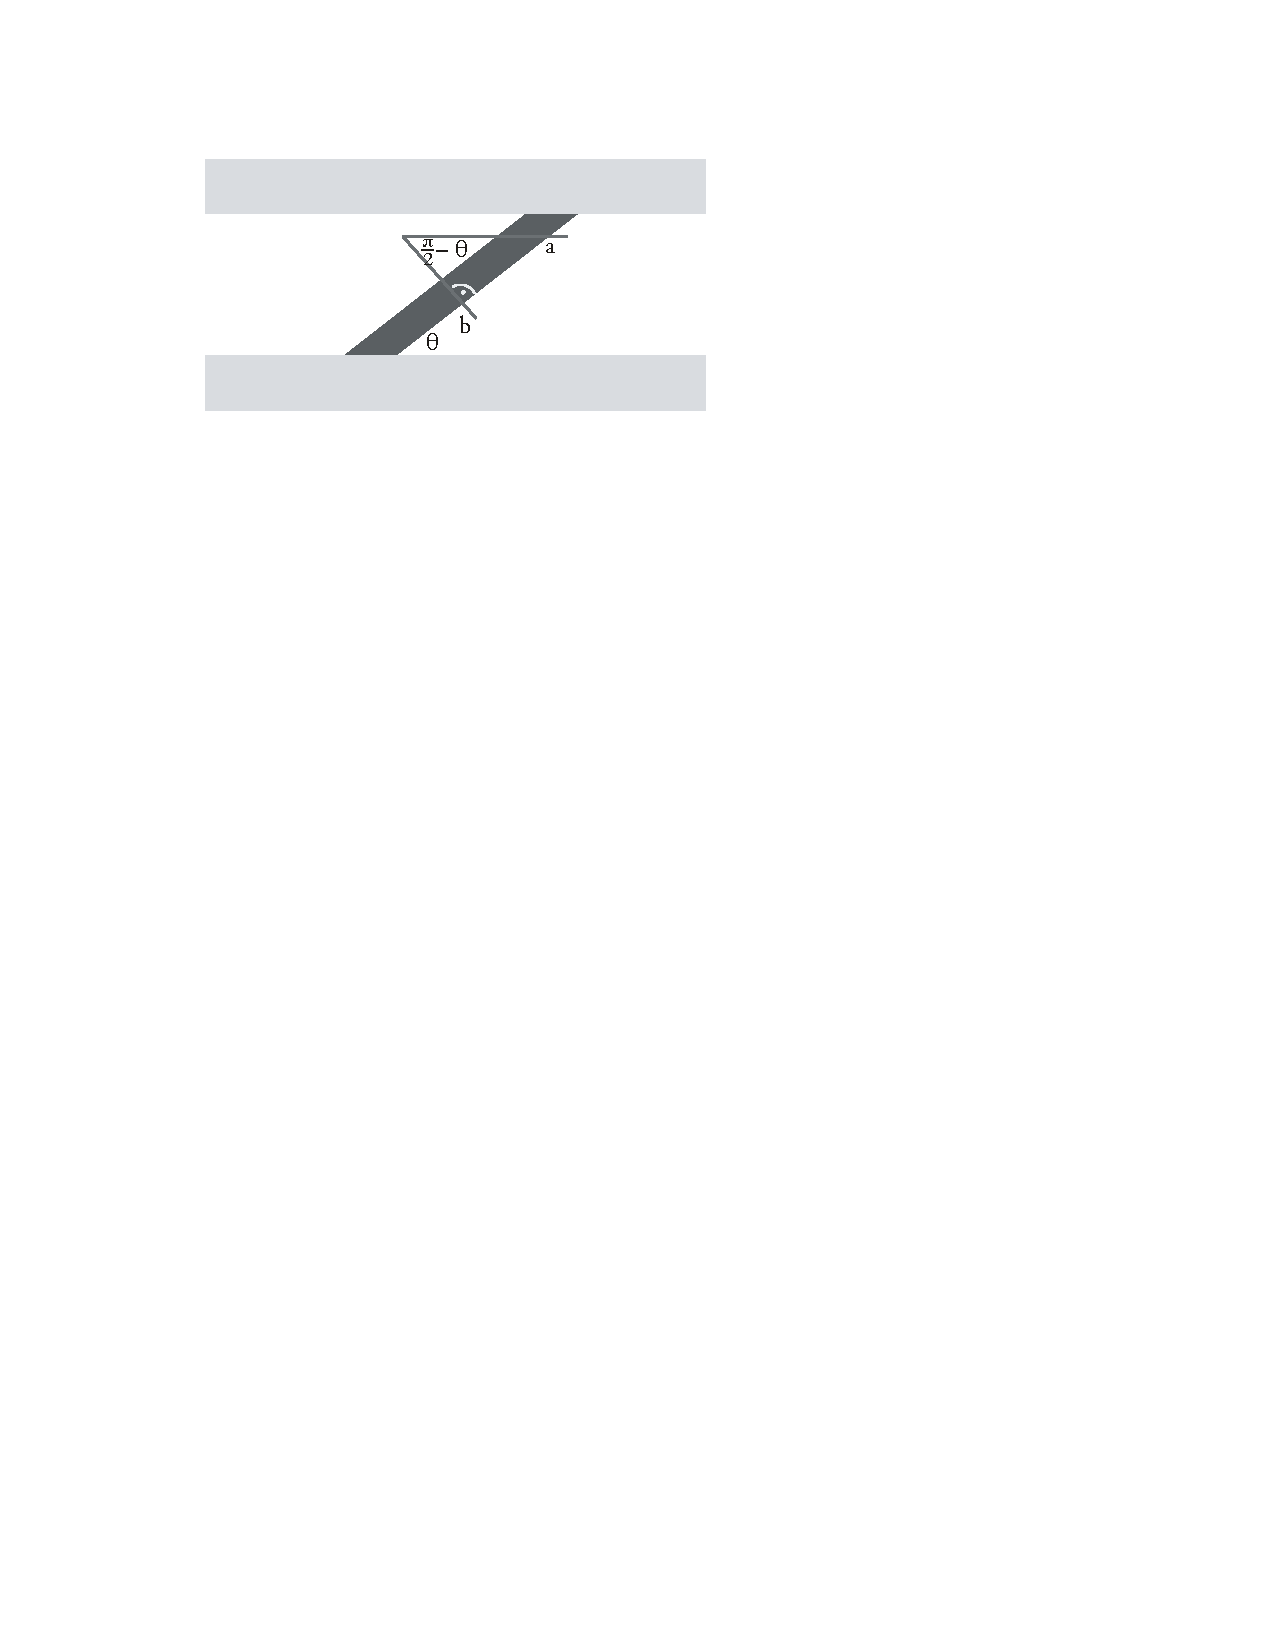
\includegraphics[width=0.6\linewidth]{images/linewidth}
\end{center}
\caption{\label{fig:linewidth}Sketch of line width assessments: (a) is showing  horizontal width, (b) shows  width orthogonal to the slope. Survey results in section \ref{results}  indicate that observers associate line width more with  orthogonal width (b) than horizontal width (a).}
\end{figure}



%XXX aspect ratio


\begin{figure*}[htbp]
\begin{center}
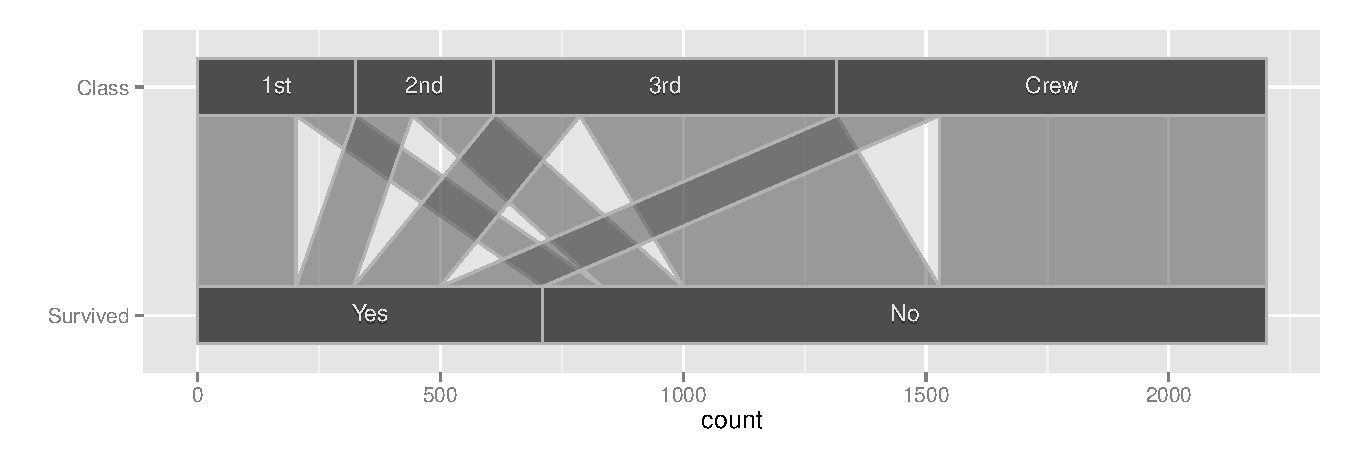
\includegraphics[height=1.5in]{images/aspect31-titanic.pdf}
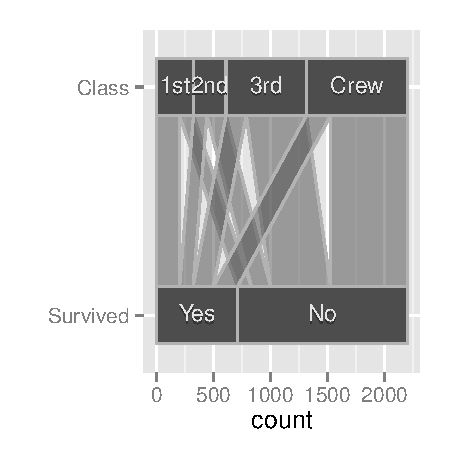
\includegraphics[height=1.5in]{images/aspect33-titanic.pdf}
\end{center}
\caption{\label{fig:aspect}Parallel sets plots of survival on the Titanic by class. Different aspect ratios  seemingly change the thickness of line segments, compare e.g. number of survivors in 3rd class and in the crew. }
\end{figure*}



The perceived slope of a line very much depends on the aspect ratio of the corresponding plot -- changing the height to width ratio of a display  will change our perception of the corresponding line widths, if they are not adjusted for the slope \cite{cleveland:1984}. This finding is not new, but its strength on our perception is surprising, as can be seen in the example of  figure \ref{fig:aspect}.  Again, survival and class membership on the Titanic is shown; the same parallel sets plot is shown twice in this figure, but with very different aspect ratios: in the  plot on the left the number of surviving 3rd class passengers seems to be about twice as big as the number of survivors among crew members, whereas in the plot on the right the lines have about equal (orthogonal) width. Obviously, this is not due to a change in numbers.

For parsets-style displays, the audience has {\it area of the line segment} an alternate visual cue when evaluating frequencies. Because height (or width for a rotated display) of  line segments is constant across the display, the width of a particular  segment is proportional to its area. We can therefore employ area comparisons as a proxy or to augment line width evaluations. 
However, existing literature suggests that this method of comparison is particularly  prone to errors in two scenarios commonly seen in parallel sets: (1) extreme aspect ratios of the rectangular shape \cite{heer:2010} %occupied by thick line segments 
and (2) when comparing rectangles rotated relative to each other \cite{kong:2010}. 
This incorrect perception and comparison of areas distorts the message readers discern from the graph. %additional contextual evidence that reinforce and strengthen distortion introduced by the line width illusion.


% needed in second column of first page if using \IEEEpubid
%\IEEEpubidadjcol
\section{Related work}
%XXX Description of hammock plots and example

Hammock plots, introduced by M Schonlau in \cite{schonlau:2003}, provide an alternative to parallel sets that is adjusted for the line width illusion. This is done by  adjusting the --horizontal-- line width by  a factor of $\sin \theta$, as discussed in equation (\ref{adjust}). This adjustment makes the perceived --orthogonal-- line width to be proportional to the number of observations it represents. 
 Figure \ref{hammock} shows an example of a four dimensional hammock plot of the Titanic data. From top to bottom Class, Gender, Survival, and again Class are shown. 
\begin{figure}
%cols <- c(brewer.pal(name="Blues", 6)[-c(1,2)], rev(brewer.pal(name="Oranges", 3)[-1]), rev(brewer.pal(name="Greens",3)[-1]))
%ggparallel(names(titanic)[c(1,4,2,1)], order=c(0,1,1,0), method="hammock", ratio=.25, text.angle=0, titanic, weight="Freq") +
%  scale_fill_manual(values=cols, guide="none") +
%  scale_colour_manual(values=cols, guide="none") + coord_flip() 
%ggsave("hammock-titanic.pdf", width=6, height=8)
\centering
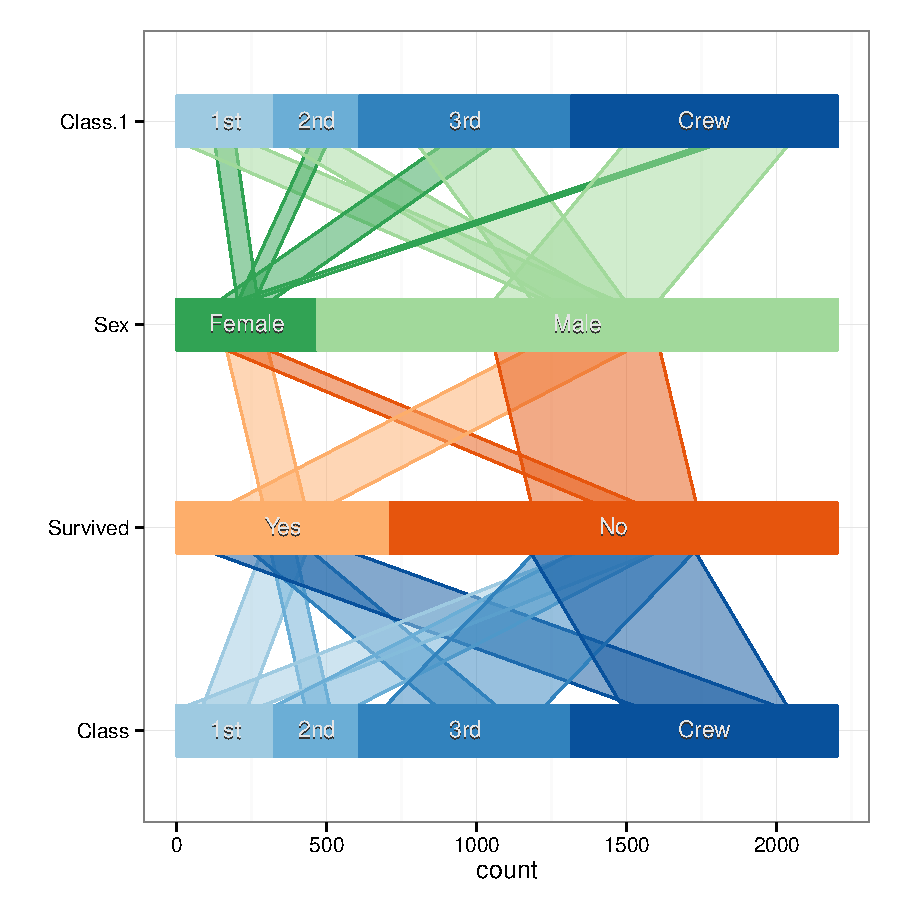
\includegraphics[width=\linewidth]{images/hammock-titanic}
\caption{\label{hammock} Hammock plot of the relationship between Class and Survival on the Titanic. }
\end{figure}

Similarly to the parallel sets plot, the bars are divided according to class membership numbers.  Lines connect categories between neighboring variables, orthogonal line widths are representing the number of individuals in each combination. Unlike the parallel sets, the lines start from the middle of the bin and connect to the middle of the other variable's bins. 

The graph shows that barely any women were in the crew, while male crew members make up the second largest contingent overall. Overall a few more men survived than women. Proportionally the situation is much different -- a much higher percentage of women survived than men. While more first class passengers survived than not, the  survival chances of second class passengers were about fifty-fifty. For third class passengers and crew members fewer members did  survive than not. 

As the adjustment of line widths is made with respect to the angle $\theta$, which itself depends on the aspect ratio of a plot, we need complete control over these properties of the plotting device when constructing hammock plots  -- in our implementation (see below for details) we have dealt with this issue by fixing the aspect ratio. This is problematic in some situations, where the rendering has to be done without knowledge of the plotting device. 

\subsection{Reverse linewidth}
A problem that arises in evaluating hammock plots is that if an observer focuses on horizontal line width  the plots suffer from a {\it reverse line width illusion}:  judging the number of survivors by class in figure \ref{hammock} based on horizontal line width  results in an ordering of (largest to smallest) Crew, 3rd, 1st, and 2nd -- which is not correct either. %Using horizontal width is inviting, since the lines are centered around the middle of a level, im
Because the lines are centered around the middle of each level, a contextual coordinate system is imposed that encourages comparisons of horizontal width. However, horizontal width alone is not proportional to underlying data. 

[[ If only h-width is considered, the graph has a lie factor; can we quantify this amount in terms of theta? ]]
%
%\section{Overview}
%From previous work \cite{cleveland:1984, tufte, wainer:2000, robbins:2005, heer:2010, kong:2010}, we may conclude that numerically accurate representations of data
%are subject to distortion due to perceptual limitations. In particular,
%the width of a single line of some thickness or the distance between two lines of minimal thickness is 
%subject to the \emph{line width illusion} even though the depiction is numerically sound.
% Furthermore, design choices during implementation \cite{schonlau:2003} may
%reduce the impact of such limitations.
%%

\section{Common angles}


\subsection{Construction}


\begin{figure}[htbp] %  figure placement: here, top, bottom, or page
%ggparallel(names(titanic)[c(1,4,2,1)], order=c(0,1,1,0), titanic, weight="Freq", text.angle=0) + 
%  scale_fill_manual(values=cols, guide="none") +
%  scale_colour_manual(values=cols, guide="none") + coord_flip() 
%ggsave("ca-titanic.pdf", width=6, height=6)
   \centering
   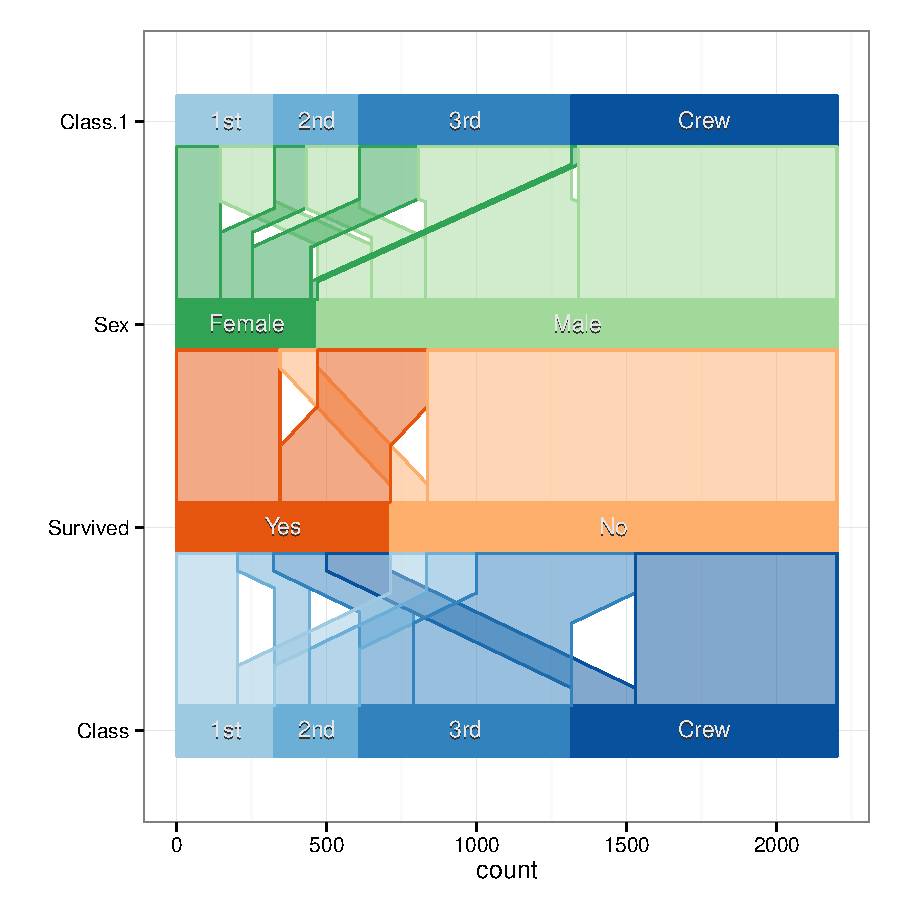
\includegraphics[width=\linewidth]{images/ca-titanic} 
   \caption{ \label{fig:ca-titanic} Common angle plot of the Titanic data. }
  \end{figure}

Figure \ref{fig:ca-titanic} shows a common angle plot of the same data as the hammock plot.

As in the previously discussed display types ribbons are drawn between categories with widths  that are proportional to  the number of records they represent.

In order to ensure that  widths of all bands are  comparable without any distortion, their slopes  are artificially made the same in the following manner: 
assuming a vertical display as shown in figure \ref{fig:ca-titanic}, we modify  the connecting bands between  categories from a straight band  to a combination of a vertical  segment, a  segment under a pre-specified angle $\theta$, followed by another vertical  segment.  
The pre-specified angle $\theta$ (between the line and the vertical band) is given as --at most-- the angle of the longest connecting line between two categories of neighboring variables. 
This makes the width of ribbons  comparable without being affected by the distortion, as all ribbons are sharing at least one segment under the same angle. 


\section{Usability Testing}
\subsection{Test}

To determine the effectiveness of the common angle plot, we conducted a user experiment in form of a survey asking participants to provide responses regarding the structure in two data sets with predominantly categorical variables.
For each data set, participants were asked to provide responses for three tasks:

Task I: simple comparison task, chosen to be unaffected by any illusion. Performance on this task should be comparable across the designs
Task II: comparison, affected by the line width illusion or its reverse. 
Task II: ordering task comprised of multiple comparisons, some of which are affected by either illusion.
  
Each participant was exposed to two of the three types of displays, one for all three tasks related to the same data set.
 
This resulted in six different survey administrations, with a crossover design as shown in Table \ref{tab:designs} that allows us to compare designs across different questions and data sets, and  simultaneously adjust for individuals' different skill sets.

\begin{table}[htbp]
\centering
\begin{tabular}{rrrrrrr}
Titanic Data & PS & CA & Ham & PS & CA & Ham \\ 
Pathway & CA & PS & PS & Ham & Ham & CA \\ \hline
\#responses &  8 (9) &  6 (7) &  8 (9) &  6 (7) & 10 (11) & 8 (8)\\ 
\end{tabular}
\caption{\label{tab:designs} Overview of study design and participation numbers. The number in parenthesis indicates the number of participants completing the first block, but not the second.}
\end{table}


\subsection{Results}

Answers for each question on the survey were assessed for correctness, and coded in binary variables of 1s and 0s, which we use to investigate performance of different designs. 

%In a first model, $M1$, we are only interested in the overall difference in performance between designs. We can express this as a model of the form
%\begin{equation}\label{model1}[M1]
%\quad\quad g(P(y_i=1)) = \mu + d_{j(i)} + u_{k(i)} + \varepsilon_i \quad\quad
%\end{equation}
%where $P(y_i=1)$ is the probability that the $i$th response is correct, for $i = 1, ..., n$. $g(.)$ is the transformation (link function) of the response. Here, we make use of the logit link, i.e.
%\begin{eqnarray*}
%g(P(y_i=1)) &=& \text{logit } P(y_i=1) = \\
%&=& \log P(y_i=1) - \log P(y_i=0).
%\end{eqnarray*}
%$d_{j(i)}$ is the parameter measuring the effect of design $j$ ($j = C, H, P$ for \underline{C}ommon Angle, \underline{H}ammock plot, and \underline{P}arallel sets plot), $u_{k(i)}$ is the effect of participant's $k$ individual skills in evaluating these plots, $k \in \{1, ..., 52\}$. The assumption is that skills are independent and normally distributed with an expected value of zero and a variance of $\sigma_u^2$.
%$\varepsilon_i$ is, similarly to a regular linear model, assumed to be independently distributed according to a normal distribution with mean of zero and variance $\sigma^2$.



%Table \ref{coef1} gives an overview of the model coefficients and their estimates. The effect of the common angle plot is used as a baseline, i.e all the effects shown are differences with respect to the performance of common angle plots. Both hammock plots and parallel sets  have negative effects on the correctness of the response. This indicates a significantly worse performance of these designs than under the common angle plot.

Table \ref{raw} shows percentages of correctness for each design and each question. Bold numbers indicate significantly different (worse) performance of a design compared to the common angle plot based on an anova model adjusted for multiple testing and individual's abilities. 


All models are fit in the {\tt lme4} package \citep{lmer} within the software frame work of {\tt R} 2.15.1 \citep{R}.


The observed results are in line with our expectations:
as we aimed for, task I does not show any significant differences between the designs and has overall the highest percentage of correctness reflecting its low difficulty level.
Parsets were affected the most by the line width illusion and show significantly worse performance for tasks II and III in both data sets. 
Hammock plots led to significantly worse performance than common angle plots in the two questions that were affected by the inverse line width illusion, while they show equal performance as common angle plots for the other questions. For task III in the pathway data,  hammock plots showed the best performance  across designs-- but this  does not  constitute a significant difference to the performance of the common angle plot.

%%xtable(summary(m1)@coefs)
%% latex table generated in R 2.15.1 by xtable 1.7-0 package
%% Fri Oct 12 09:08:11 2012
%\begin{table}[ht]
%\begin{center}
%\begin{tabular}{lrrrrl}
%  \hline
% & Estimate & Std. Error & z value & Pr($>$$|$z$|$) & \\ 
%  \hline
%$\mu$ & 1.72 & 0.24 & 7.04 & 0.00 & ***\\ [5pt]
%  $d_C$& 0.00 & -- & -- & -- \\ 
%  $d_H$ & -0.86 & 0.32 & -2.65 & 0.01 & ** \\ 
%  $d_P$ & -1.31 & 0.32 & -4.07 & 0.00 & ***\\ 
%   \hline
%\multicolumn{5}{l}{Signif. codes:  0 `***' 0.001 `**' 0.01 `*' 0.05 `.' 0.1 ` ' 1 }
%\end{tabular}
%\end{center}
%\caption{\label{coef1} Model fit for $M1$ measuring correctness of answers in the survey. The common angle plot is used as baseline -- both hammock plots and, to a larger degree, parallel sets, show a significantly worse performance. }
%\end{table}
%

%xtable(round(acast(survey, qu~design, fun=mean, value.var="correct")*100,3), digits=1)
% latex table generated in R 2.15.1 by xtable 1.7-0 package
% Fri Oct 12 11:21:19 2012
\begin{table}[ht]
\begin{center}
\begin{tabular}{llrrrr}
  \hline
Task & Data & \multicolumn{3}{l}{Design} \\
& & common & hammock & parset \\ 
  \hline
 I & Titanic & 86.0 & 76.5 & 81.2 \\ 
 & Pathway & 93.8 & 83.3 & 82.2 \\ [3pt]
 II & Titanic  & 63.2 & {\bf 5.9} & {\bf 12.5} \\ 
 & Pathway  & 68.8 & 68.8 & {\bf 6.7} \\ [3pt]
 III & Titanic  & 73.7 & {\bf 17.6} & {\bf 25.0} \\ 
 & Pathway  & 75.0 & 87.5 & {\bf 53.3} \\
   \hline
\end{tabular}
\end{center}
\caption{\label{raw} Raw percentages of correctness of responses for each question and design. Bold numbers indicate significant difference from common angle plot performance. }
\end{table}

%Model $M2$ extends the first model by including both  effects for individual questions and the interaction effects with each design in the following form:
%\begin{eqnarray}\nonumber
%[M2]  \ \ \qquad g(P(y_i=1)) =  \qquad\qquad\qquad\qquad\qquad&&\\ \label{m2}
%\mu + d_{j(i)}  + q_{q(i)} + p_{j(i),q(i)} + u_{k(i)} + \varepsilon_i 
%\end{eqnarray}
%$d_{j(i)}$ is the parameter measuring the effect of design $j$ ($j = C, H, P$ for \underline{C}ommon Angle, \underline{H}ammock plot, and \underline{P}arallel sets plot), $u_{k(i)}$ is the effect of participant's $k$ individual skills in evaluating these plots, $k \in \{1, ..., 52\}$. The assumption is that skills are independent and normally distributed with an expected value of zero and a variance of $\sigma_u^2$.
%$\varepsilon_i$ is, similarly to a regular linear model, assumed to be independently distributed according to a normal distribution with mean of zero and variance $\sigma^2$.
%$q$ indicates the effects on performance for  each question, where $q(i)$ describes one of the questions $\{A1, A2, A3, B1, B2, B3\}$. $p$ is the parameter for the interaction effect of design and question, its index is a tuple consisting of a combination of a question and design. 
%
%%Figure \ref{fitted.m2} gives an overview of the goodness of fit of model $M2$ -- histograms of fitted values are drawn facetted by levels of the dependent variable. For correct responses fitted values are highly left skewed, with most values  above 0.5. For wrong answers we see a symmetric, if not quite as clear-cut picture: fitted values are skewed right. 
%%Overall, Model $M2$ is a significant improvement over model $M1$ (a corresponding log-likelihood ratio test is significant at a level of $<\!\!\!< 10^{-8}$).
%%Table \ref{model2} shows an overview of the  parameters and their estimates for model $M2$. After adjusting for individuals' skills parallel sets performs significantly worse than common angle plots in three of the six questions. 
%%
%%\begin{figure}
%%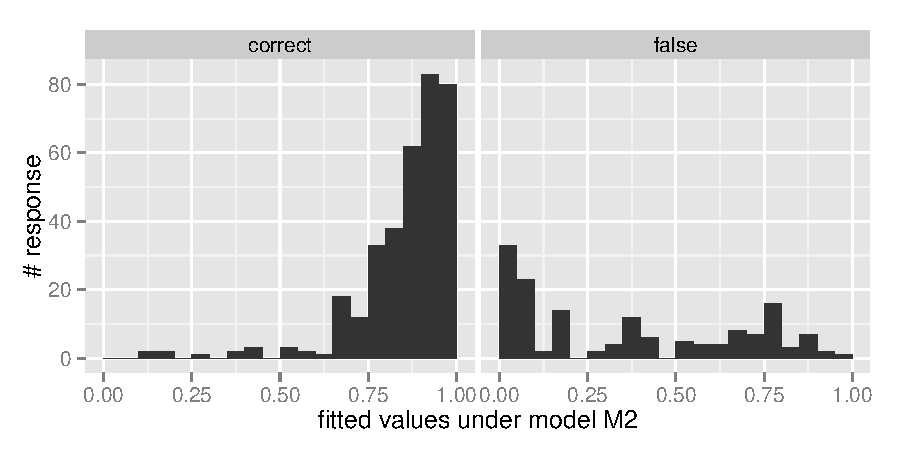
\includegraphics[width=\linewidth]{fitted-m2}
%%\caption{\label{fitted.m2} Histograms of fitted values under model $M2$, facetted by actual performance of participants. On the left, correct responses are shown. The histogram of fitted values is skewed to the right, with most values above 0.5. The histogram on the right corresponds to wrong answers. There are fewer wrong answers, and they tend to have low fitted values, but there are more false positives among them than false negatives for correct answers. }
%%\end{figure}
%
%% xtable(summary(m4)@coefs)
%% latex table generated in R 2.15.1 by xtable 1.7-0 package
%% Fri Oct 12 09:12:32 2012
%\begin{table}[ht]
%\begin{center}
%\begin{tabular}{rrrrrl}
%  \hline
% & Estimate & Std. Error & z value & Pr($>$$|$z$|$) & \\ 
%  \hline  
%$\mu$ & 2.68 & 0.61 & 4.35 & 0.00  & ***\\ [5pt]
%Design\\
%  $d_C$ & 0.00 & -- & -- & -- \\ 
%  $d_H$ & -1.06 & 0.83 & -1.28 & 0.20  \\ 
%  $d_P$ & -0.57 & 0.86 & -0.66 & 0.51 \\ [5pt]
%Questions\\
%  $q_{A1}$ & 0.00 & -- & -- & -- \\ 
%  $q_{A2}$  & -1.85 & 0.74 & -2.50 & 0.01 &* \\ 
%  $q_{A3}$  & -1.11 & 0.77 & -1.44 & 0.15 \\ 
%  $q_{B1}$ & 0.55 & 0.96 & 0.58 & 0.56 \\ 
%  $q_{B2}$  & -1.69 & 0.88 & -1.91 & 0.06 &. \\ 
%  $q_{B3}$  & -1.31 & 0.92 & -1.43 & 0.15 \\ [5pt]
% 
%Interaction \\
%$p_{H, A1}$ &  0.00 & -- & -- & -- \\
%$p_{P,A1}$ &  0.00 & -- & -- & -- \\
%$p_{H, A2}$ &  -3.29 & 1.55 & -2.13 & 0.03 & *\\ 
%$p_{P,A2}$ & -3.03 & 1.33 & -2.28 & 0.02 &*\\ 
%$p_{H,A3}$ &-2.61 & 1.17 & -2.24 & 0.03  & * \\ 
%$p_{P,A3}$ & -2.60 & 1.16 & -2.23 & 0.03 &*\\ 
%$p_{H,B1}$ &-0.26 & 1.21 & -0.22 & 0.83 \\ 
%$p_{P,B1}$ &-0.81 & 1.24 & -0.65 & 0.51 \\ 
%$p_{H,B2}$ & 1.03 & 1.22 & 0.85 & 0.40 \\ 
%$p_{P,B2}$  & -3.48 & 1.63 & -2.14 & 0.03 &*\\ 
%$p_{H,B3}$ & 1.97 & 1.37 & 1.44 & 0.15 \\ 
%$p_{P,B3}$ & -0.62 & 1.26 & -0.50 & 0.62 \\   
%   \hline
%\multicolumn{6}{l}{Signif. codes:  0 `***' 0.001 `**' 0.01 `*' 0.05 `.' 0.1 ` ' 1 }
%\end{tabular}
%\end{center}
%\caption{\label{model2} Model fit for $M2$ measuring correctness of answers in the survey, detailing performance of designs on each question. All design comparisons are with respect to the common angle plot. }
%\end{table}
%

\begin{figure}
\centering 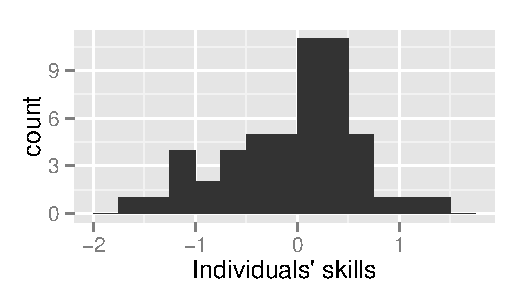
\includegraphics[width=.7\linewidth]{hist-skills}
\caption{\label{skills}Histogram of the predictions of subject-specific skills. }
\vspace{-0.2in}
\end{figure}	
Figure \ref{skills} shows an overview of the predicted skill for each participant under model $M2$. Skills are quite varied between  -1.52 and  1.34, but
a Kolmogorov-Smirnov test  does not show significant deviation from a normal assumption ($p$-value = 0.089).
On the scale of the dependent variable the range in individuals' skills translates to a $17.5 = e^{1.34 - (-1.52)}$ fold increase in the probability of answering a question on the survey correctly between participants with the best skill set and the worst.

In the next section we will investigate the results from the survey in further detail for some questions, and highlight the link to the line width illusion and its inverse.

\subsubsection{Evidence for line width illusions}

Question $A2$ asked participants to order  class levels  according to the number of survivors, fewest to highest. There are 4! = 24 distinct orderings of the levels, corresponding to all permutations of length 4. Some orderings are closer to one another than other orderings.  To quantify distance between each pair of permutations, the Cayley distance is defined as the minimal number of transpositions (i.e. swaps of two elements) necessary to transform one permutation into another.

%The Cayley distance defines a way to quantify the distance between  each pair of permutations; the Cayley distance is defined as the minimal number of transpositions, i.e. swaps of two elements,  necessary to transform one permutation into the other.
This distance is used to define a graph on the space of all permutations: let all permutations be nodes of the graph; for each two permutations with a Cayley distance of one, we add an edge between these nodes to the graph. The resultant regular graph of degree six, i.e. each  node is connected to six other nodes. Between any two nodes, the Cayley distance is then given as length of shortest connecting path shown on the graph.
%The Cayley distance between any two nodes is then given as the length of the shortest connecting path between these two nodes through the graph.
Figure \ref{cubes} shows an overview of the permutation space together with an overview of the survey results. Each permutation is represent by one dot. 

The colored dots on top of the graph correspond to the responses from the survey - the size of the dots is proportional to the number of observers choosing this particular ordering. It becomes obvious from the three graphs in figure \ref{cubes} that
the answers to different designs occupy quite different regions, while answers based  on the same design are quite close --  usually separated by only one edge. 

The correct ordering, as well as the orderings assuming the line width illusion and its reverse are marked with symbols. Answers for the common angle plot are centered around the correct answer, while responses to parallel sets are cluster around the response corresponding to the line width illusion. Due to the small number of responses to the hammock design a clear clustering of the answers is not recognizable, but the answer for the inverse line width illusion is among the responses. Table \ref{a2} gives an overview of all responses to question $A.2$. 

\begin{table}[ht]
\begin{center}
\begin{tabular}{rrrrl}
Order  & CA & H & PS\\
  \hline
  Crew, 1st, 3rd, 2nd &  &  2 &  \\ 
  2nd, 1st, 3rd, Crew &  &  6 &  & inverse illusion \\ 
   Crew, 3rd, 1st, 2nd &  &  1 &  1 \\ 
  2nd, 3rd, 1st, Crew & 1 & 7 & 1 \\ 
  2nd, 3rd, Crew, 1st & 12 &  1 &  2 & correct\\ 
  Crew, 3rd, 2nd, 1st &  2 &  &  \\ 
  3rd, 2nd, Crew, 1st &  1 &  &  \\ 
  1st, 2nd, 3rd, Crew &  1 &  &   \\ 
  1st, 3rd, Crew, 2nd &  1 &  &  2 \\ 
  Crew, 2nd, 3rd, 1st &  &  & 6 &  line width illusion\\  
  1st, 3rd, 2nd, Crew &  &  &  2 \\ 
  2nd, Crew, 3rd, 1st &  &  &  3 \\ 
   \hline
  Total & 18 & 17 & 16 \\ 
   \hline
\end{tabular}
\end{center}
\caption{\label{a2} Responses to question $A.2$: order levels of Class by the number of survivors (smallest to largest). }
\end{table}

%
Common angle plots show the best performance in terms of correctness (66.7\% on 18 responses), compared to a correctness of 11.8\% for parallel sets plots on 16 responses, indicating a significantly better performance of common angle plots at a level of 0.0027, based on a Mantel-Haenszel test (the difference in performance to hammock plots is also significant at a level of 0.0006; but there is no significant difference in correctness between hammock plots and parallel sets.).
While the intuitive assessment of lines by their width orthogonal to their direction is well known, it is surprising to see its strength: in this particular setting, it is strong enough to `shrink' the horizontally widest line for 6 out of 16 participants by at least  44\%, from 212 to below 118, and a further 3 participants perceived the shrinking to below 178, which constitutes a distortion of at least 16\%.

\begin{figure*}
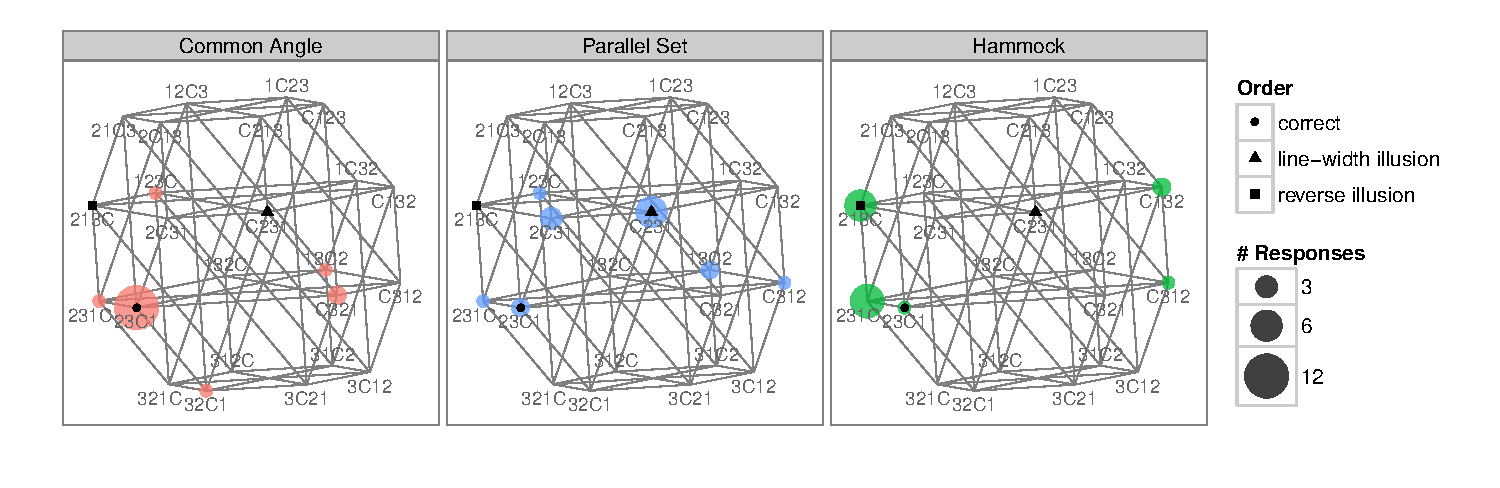
\includegraphics[width=\linewidth]{cubes}
\caption{Answers to question A.2 -- each node corresponds to a single ordering of the levels in variable 'Class'. Lines are drawn between orderings that are only one swap of levels apart. The colored dots show responses from the survey, their sizes depend on the number of responses for each ordering. }
\label{cubes}
\end{figure*}

Responses to question A.3 exhibit a similar pattern, see table \ref{a3}.

\begin{table}[ht]
\begin{center}
\begin{tabular}{rrrrl}
Order & CA & H & PS\\
  \hline
c, b, a &  &  2 &  \\
a, b, c &  1 &  12 &  & inverse illusion\\ 
a, c, b & 13 &  3 &  4 & correct\\ 
b, c, a &  2 &  &  1 \\ 
c, a, b &  2 &  & 9 & line width illusion\\ 
b, a, c &  &  &  2 \\ 
 \hline
  Total & 18 &  17 & 16 \\ 
   \hline
\end{tabular}
\end{center}
\caption{\label{a3}Responses to question A.3: order combinations from smallest to largest, where 'a' is first class female, 'b' are male survivors, and 'c' are crew survivors. }
\end{table}
  
\begin{table}[ht]
\begin{center}
\begin{tabular}{clrrrl}
  Qu & Design & \rotatebox{90}{Correct} & \rotatebox{90}{Incorrect} & \rotatebox{90}{No Answer}   & Reason\\ \hline
  \hline
1 & common &   14 &  2 &   0 \\ 
   & hammock &   15 &  0 &   1 \\ 
 & parallel &   7 &   7 &   0 & line width illusion\\ \hline
2 & common &  16 &   0 &   0 \\ 
& hammock &   9 &   7 &   0 & inverse illusion\\ 
& parallel &  14 &   0 &   0 \\ \hline
3& common &  15 &   1 &   0 \\ 
& hammock &  16 &   0 &   0 \\ 
& parallel &  14 &   0 &   0 \\ 
   \hline
\end{tabular}
\end{center}
\caption{\label{tab:b1}Responses to question set B.1 }
\vspace{-0.25in}
\end{table}


Table \ref{tab:b1} shows a summary to the  three questions of $B.1$ with possible answers ``agree", ``disagree", and ``don't know".
The first two questions are  examples, where the line width illusion, and its reverse will lead to answers that differ from the correct answer. Parallel sets  are susceptible to the line width illusion, while hammock plots suffer from the reverse. The data shows that in about 50\% of the responses we can see this difference. 7 out of 14 answers for the parallel sets plots in question 1 deviate from the correct answer, and 7 out of 16 responses corresponding to hammock plots in question 2 show the wrong answer.


\subsubsection{Opinion on common angle plots}
Answers to the question of `which chart did you like better?' are shown in table \ref{tab:prefer}. There is a pretty clear endorsement in favor of common angle plots versus the other two types of displays.
Asked for a reason for their preference over parallel sets, 8 participants cited a facilitated comparison of width, area or ``size", 3 saw the common angle plots as preferable, and the remaining answers related to a 'more logical' structure or generally 'easier' choice.
Reasons for not preferring common angle plots boiled down to a preference for straight lines. This purely aesthetic preference is deeply rooted and in our opinion the biggest challenge for common angle plots.
% latex table generated in R 2.15.1 by xtable 1.7-0 package
% Wed Oct 31 10:28:55 2012
\begin{table}[ht]
\begin{center}
\begin{tabular}{cccrrr}
  \hline
&\multicolumn{5}{r}{Which chart did you like better?}\\
&&& Chart 1 &  Chart 2 \\ 
  \hline
  PS &vs&  {\bf CA} & 2 & \bf 6 \\ 
 {\bf  CA} & vs &  PS & \bf 4 & 2 \\ 
  H & vs &   {\bf  CA} & 3 & \bf 5 \\ 
   {\bf  CA} & vs &  H & \bf 8 & 2 \\ 
  H & vs &  PS & 3 & 5 \\ 
  PS & vs &  H & 1 & 5 \\ 
   \hline
\end{tabular}
\caption{\label{tab:prefer} Preferences for first or second chart across all six combinations of questions and chart types. }
\vspace{-0.3in}
\end{center}
\end{table}

\section{Conclusion}
The conclusion goes here.





% if have a single appendix:
%\appendix[Proof of the Zonklar Equations]
% or
%\appendix  % for no appendix heading
% do not use \section anymore after \appendix, only \section*
% is possibly needed

% use appendices with more than one appendix
% then use \section to start each appendix
% you must declare a \section before using any
% \subsection or using \label (\appendices by itself
% starts a section numbered zero.)
%


\appendices
%\section{Proof of the First Zonklar Equation}
%Appendix one text goes here.
%
%% you can choose not to have a title for an appendix
%% if you want by leaving the argument blank
%\section{}
%Appendix two text goes here.


% use section* for acknowledgement
\section*{Acknowledgment}


The survey for this study was carried out with approval from  IRB-ID 12-204.


% Can use something like this to put references on a page
% by themselves when using endfloat and the captionsoff option.
\ifCLASSOPTIONcaptionsoff
  \newpage
\fi



% trigger a \newpage just before the given reference
% number - used to balance the columns on the last page
% adjust value as needed - may need to be readjusted if
% the document is modified later
%\IEEEtriggeratref{8}
% The "triggered" command can be changed if desired:
%\IEEEtriggercmd{\enlargethispage{-5in}}



%% if specified like this the section will be ommitted in review mode
\acknowledgments{
The survey for this study was carried out with approval from  IRB-ID 12-204. 
}

\bibliographystyle{plain}
%%use following if all content of bibtex file should be shown
%\nocite{*}
\bibliography{references}
\end{document}